\documentclass[12pt,a4paper]{article}
\usepackage{amssymb}
%\usepackage{latexsym}
\usepackage{amsmath}
\usepackage{listings}
\usepackage{graphicx}
\usepackage{color}
\usepackage{url}
\usepackage{caption}


\captionsetup{width=.8\textwidth,font=small} 

% Stolen settings (unknown origin):
% Alter some LaTeX defaults for better treatment of figures:
% See p.105 of "TeX Unbound" for suggested values.
% See pp. 199-200 of Lamport's "LaTeX" book for details.
%   General parameters, for ALL pages:
\renewcommand{\topfraction}{0.9}	% max fraction of floats at top
\renewcommand{\bottomfraction}{0.8}	% max fraction of floats at bottom
%   Parameters for TEXT pages (not float pages):
\setcounter{topnumber}{2}
\setcounter{bottomnumber}{2}
\setcounter{totalnumber}{4}     % 2 may work better
\setcounter{dbltopnumber}{2}    % for 2-column pages
\renewcommand{\dbltopfraction}{0.9}	% fit big float above 2-col. text
\renewcommand{\textfraction}{0.07}	% allow minimal text w. figs
%   Parameters for FLOAT pages (not text pages):
\renewcommand{\floatpagefraction}{0.7}	% require fuller float pages
% N.B.: floatpagefraction MUST be less than topfraction !!
\renewcommand{\dblfloatpagefraction}{0.7}	% require fuller float pages

% remember to use [htp] or [htpb] for placement

\author{Rasmus Einarsson, Jonatan Kallus, Olof Nilsson, Joel Wilsson}
\title{Simulation of Complex Systems\\Lattice gas automata.}

\begin{document}
\maketitle

\section{Introduction.}

\section{Theory.}
The lattice gas model describes how particles move around on a lattice. Particles make discrete jumps between lattice nodes, where they may collide with each other and change directions. In the following discussion, we only consider two-dimensional lattices.

Specifically, the model consists of a lattice where each node takes on one of a finite set of states. Each state represents a configuration of particles in that site. In each time step, the nodes are updated according to a rule based on the values of the nearest neighbors. The update rule corresponds to particle collisions and movements between neighboring nodes.

Consider the example of a square lattice, where each node has four neighbors. For a particle in a node, there are four possible velocities (up, down, left, right). For each lattice node, there can be at most one particle moving in each direction. Hence, the state of a node can be encoded in four binary values indicating whether there is or is not a particle moving in each direction. See figure \ref{fig:square-state} for an illustration.

\begin{figure}[htp]
\centering
  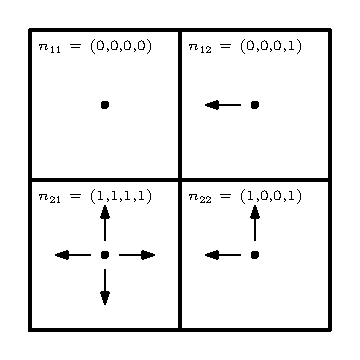
\includegraphics{figs/square-state.pdf}
\caption{Example showing the state of four nodes. Each node can be occupied by zero to four particles, one in each direction. The state $n_{ij}$ can be encoded using four binary values \{up, right, down, left\} as indicated the figure. For instance, in the upper right corner, there is one particle moving to the right. In the lower right corner, there are particles moving upwards and to the left, etc.}
\label{fig:square-state}
\end{figure}

A time step in the model is described by a mapping, where we write $n_{ij}^t$ to denote the the state of node $(i,j)$ at $t$,
\begin{equation}\label{eqn:mapping}
n^{t+1}_{ij} = f(n^t_{ij}, n^t_{i+1,j}, n^t_{i,j+1}, n^t_{i-1,j}, n^t_{i,j-1}).
\end{equation}
In theory, this map can be written down explicitly. The node $(i,j)$ and its four nearest neighbors have a total of $2^{20}\approx 10^6$ states, and these states map to the $2^4=16$ possible states $n^{t+1}_{ij}$. In other words, the map is
$
f: \{0,1\}^{20} \longrightarrow \{0,1\}^4.
$
A more practical representation is divided into two operations, propagation and collision. 

In the propagation operation, each particle moves to the next node (see figure \ref{fig:propagation}). All nodes are equidistant the lattice, which means the particles all have the same speed.

In the collision operation, collisions between particles are considered. Two particles in the same node can collide with each other, so that they change directions. With the restriction that collisions must preserve momentum, one can verify that the only allowed collision rules are the ones shown in figure \ref{fig:collision}. All other states must map to themselves in the collision operation.

The lattice gas model can be propagated by alternating between the collision and propagation operations. Applying both operators in sequence is equivalent to taking one time step according to equation \eqref{eqn:mapping}. For a complete example of a time step, see figure \ref{fig:collision-propagation}.


\section{Implementation details.}
% describe bouncing off walls, random initializations at sources... anything else?

\section{Experiments, results.}
% or should this just say ``waves''?
\subsection{Shockwaves.}
We start out with a square area, surrounded by walls, where initially each lattice site (not including walls)
is completely filled with a probability of 0.3. Completely filled means that it contains six or
four particles, if we use a hexagonal or a square lattice, respectively. After one time step,
this looks completely random, as can be seen in figure \ref{hexwaveinit}. In this figure, and the
next few figures, we used a hexagonal lattice. The effects of using a square lattice instead will be
explained in the last part of this section.

\begin{figure}[htp]
% if we change to just waves, this caption needs to be changed.
\caption{Initial conditions, after one time step, for the shockwave experiment using a hexagonal lattice.}
\centering
  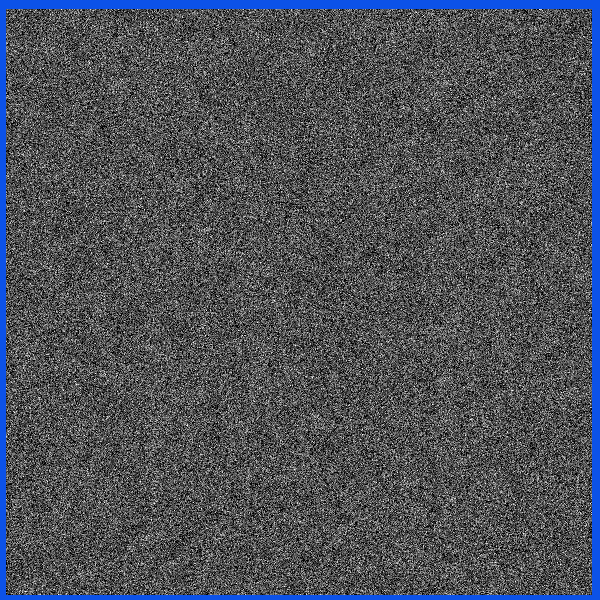
\includegraphics[width=100pt]{figs/hexwaveinit.png}
\label{hexwaveinit}
\end{figure}

By clicking the left mouse button we set a circular area of lattice sites around the mouse cursor to
be completely filled. Just like a real gas, on average these added particles move towards areas of lower
concentrations of particles, away from the spawn point (since the circular area has the highest concentration
possible). Three frames taken just after the particles were added are shown in figure \ref{hexwavestart}.

\begin{figure}[htp]
\caption{Frames demonstrating the initial phase of the shockwave.}
\centering
  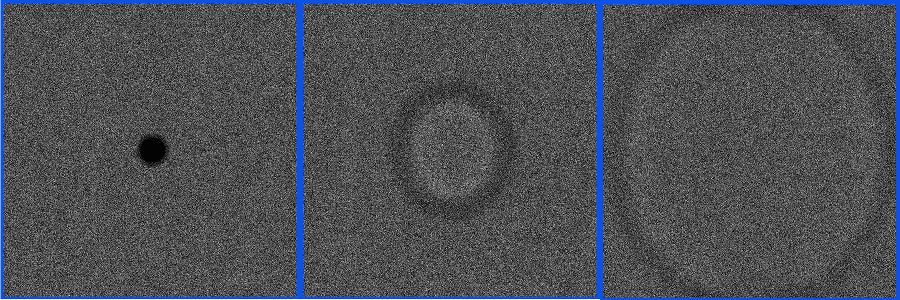
\includegraphics[width=300pt]{figs/hexwavestart.png}
\label{hexwavestart}
\end{figure}


The resulting waves bounce off against the walls, figure \ref{hexwavebounce}.
\begin{figure}[htp]
\caption{Just like real waves, the lattice gas shockwaves bounce off the walls.}
\centering
  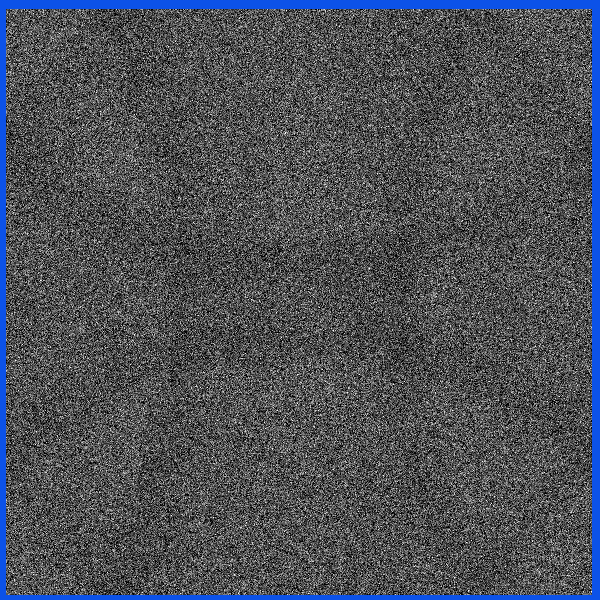
\includegraphics[width=100pt]{figs/hexwavebounce.png}
\label{hexwavebounce}
\end{figure}

Eventually, through collisions
with the other random particles in the box, the particles we added spread out and the pattern which was formed
when we filled the circular area is lost. Figure \ref{hexwaveend} shows what it looks like many time
steps later (approximately 30 seconds later, when the simulation is run on a fast computer).
We can see no trace of the shockwave.

\begin{figure}[htp]
\caption{Many updates later, the picture looks the same as before the shockwave.}
\centering
  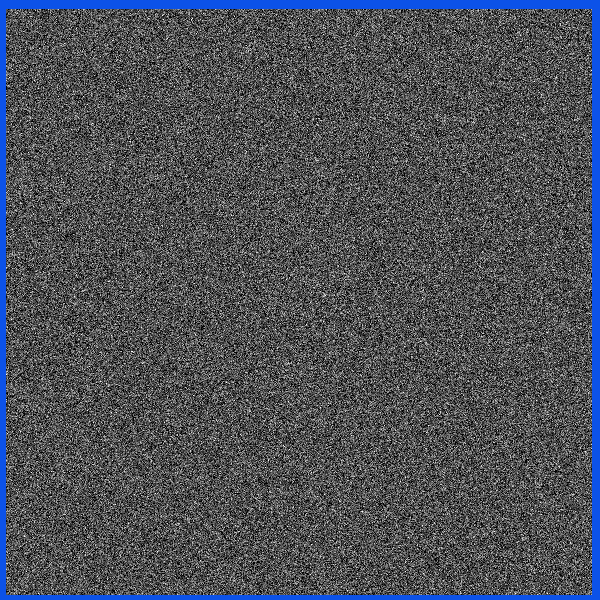
\includegraphics[width=100pt]{figs/hexwaveend.png}
\label{hexwaveend}
\end{figure}


% compare to analytical results, if possible?

If we use a square lattice instead, we still get the wave-like behaviour, figure \ref{squarewave}.
\begin{figure}[htp]
\caption{The shockwave looks similar when using a square lattice.}
\centering
  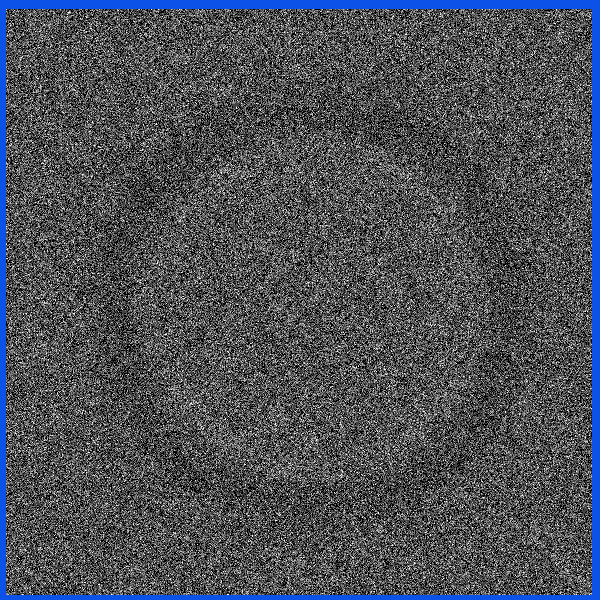
\includegraphics[width=100pt]{figs/squarewave.png}
\label{squarewave}
\end{figure}

However, the waves persist for much longer, possibly because there are fewer possible collisions.
Even after letting the simulation run for a long time after the particles were added, traces of waves
going back and forth can still be seen. Unfortunately, this is not clear from a static picture, so
it's not possible to show them in this report.

% the following is a hypothesis. it makes sense to me, but does it make sense to you?
Also, there are fewer particles in total (since each site can contain at most four particles, instead of six).
This means there are fewer possible states for the system, and therefore it has lower entropy, so patterns
(such as the non-randomly initialized circle completely filled with particles) which lower the entropy would make
a bigger relative difference than for the hexagonal lattice.

\subsection{Diffusion.}
In this experiment, we have three boxes in a row, and the gas can spread between adjacent boxes through a small
hole in the separating wall. Initially, all boxes are empty except for the first one, where each lattice site
is completely filled with particles. The initial conditions are shown in figure \ref{diffusioninit}.

\begin{figure}[htp]
% if we change to just waves, this caption needs to be changed.
\caption{Initial conditions, after one time step, for the diffusion experiment.}
\centering
  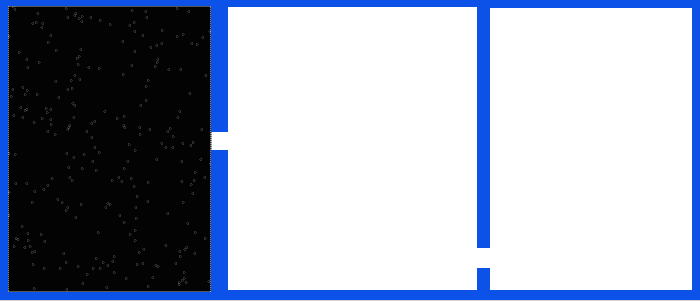
\includegraphics[width=200pt]{figs/diffusioninit.png}
\label{diffusioninit}
\end{figure}

As the simulation runs, the gas spreads first to the second box (figure \ref{diffusionbox2fill}.
\begin{figure}[htp]
\caption{Much of the gas has spread to the second box.}
\centering
  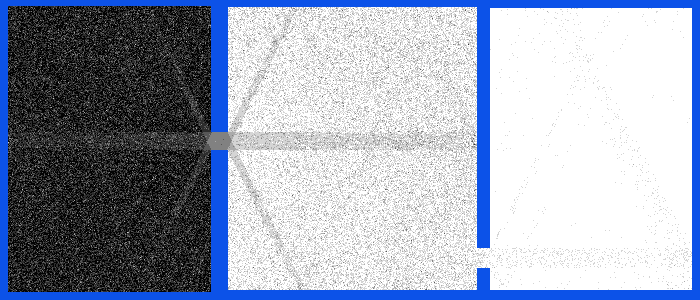
\includegraphics[width=200pt]{figs/diffusionbox2fill.png}
\label{diffusionbox2fill}
\end{figure}

Eventually, particles also start to fill up the third box (figure \ref{diffusionbox3fill}.
\begin{figure}[htp]
\caption{A while later, many particles are also found in the third box.}
\centering
  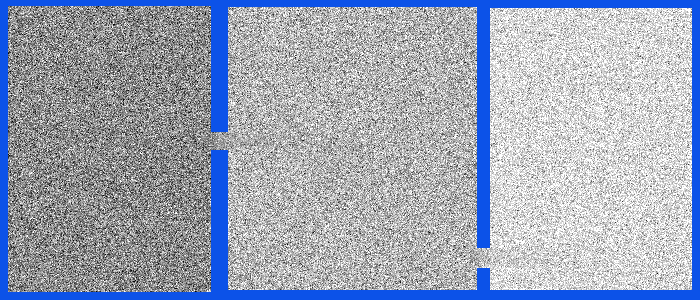
\includegraphics[width=200pt]{figs/diffusionbox3fill.png}
\label{diffusionbox3fill}
\end{figure}

Given enough time, they spread out uniformly over the whole available space, just like a real gas would.
This ``steady-state'' is shown in figure \ref{diffusionend}.
\begin{figure}[htp]
\caption{Eventually, the particle density is the same for all boxes.}
\centering
  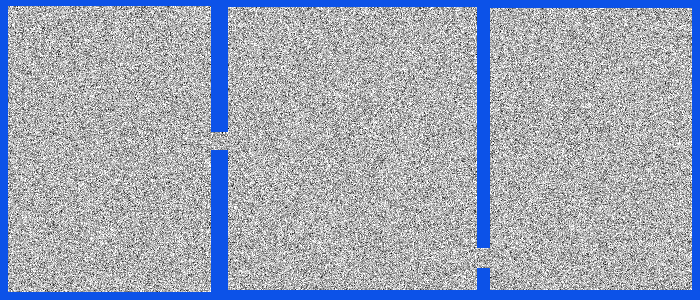
\includegraphics[width=200pt]{figs/diffusionend.png}
\label{diffusionend}
\end{figure}

We modified our program to count the number of particles in each box; see figure \ref{gascount}.
% compare to theoretical results?
\begin{figure}[htp]
\caption{Number of particles in each box as a function of the number of updates.}
\centering
  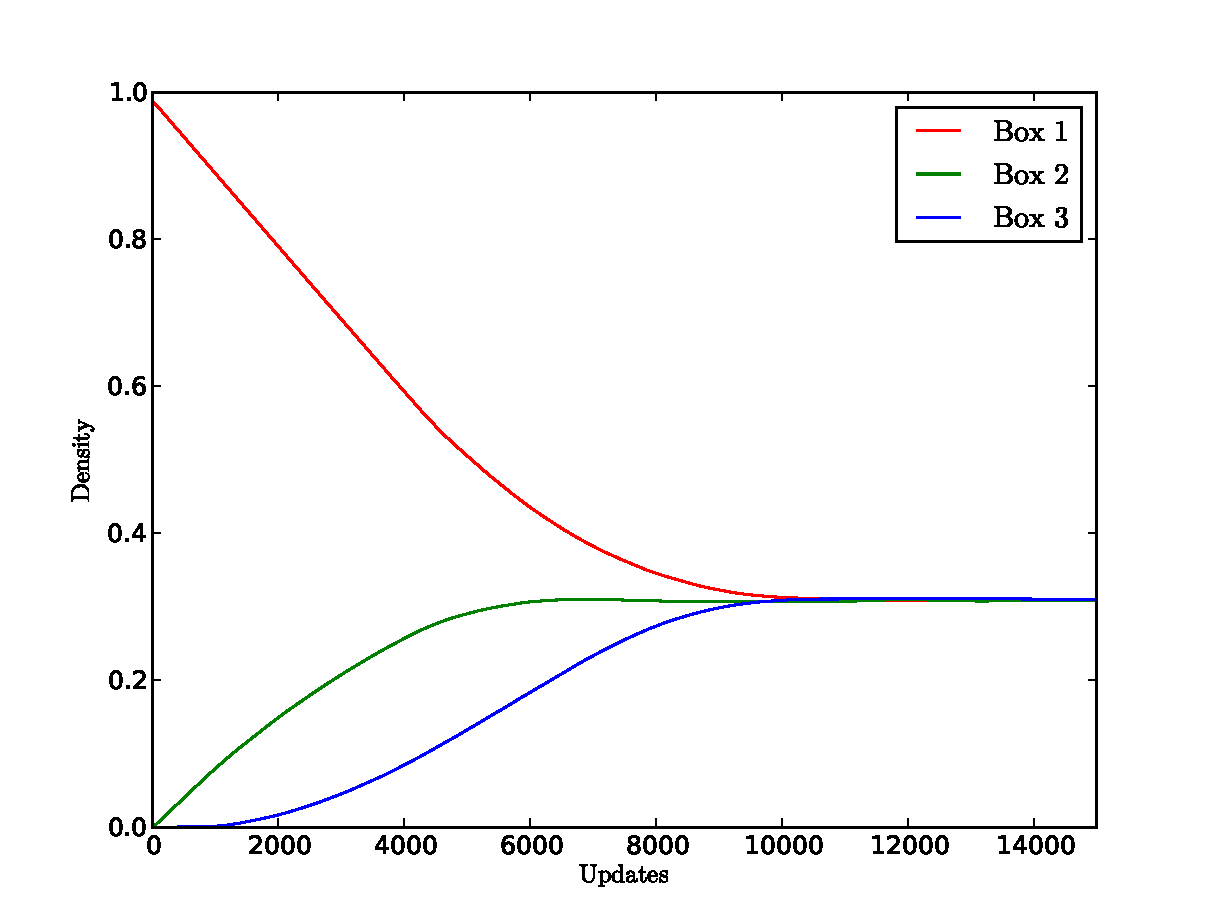
\includegraphics[width=300pt]{figs/gascount.pdf}
\label{gascount}
\end{figure}

\subsection{Flow around cylinder.}

\section{Conclusion.}

\end{document}
